% !TEX root = ../thesis.tex

\section{Data and Simulation Samples}
\label{sec:samples}

% The need for simulation samples of signal and background
This search uses the proton-proton collision data collected by the CMS detector during Run 2.
The data are collected and stored for analysis after events generate trigger primitives in the detector subsystems and are selected by the L1 Trigger and HLT as described in chapter~\ref{chap:exp}.
We also list the MC signal samples used in the analysis that are based on the BSM models of subsection~\ref{subsec:benchmark}.
Additionally, we list the MC samples that model SM background contributions to the search.

\subsection{Data Samples}

% Data samples
The data used for this work are based on three different sets over the three Run 2 years of 2016, 2017, and 2018.
For each year of Run 2, documentation is available for the luminosity measurements~\cite{CMS-PAS-LUM-17-001,CMS-PAS-LUM-17-004,CMS-PAS-LUM-18-002}.
The full dataset is divided into three sets per year, with contributions from the \texttt{SingleMuon}, \texttt{SingleElectron}, and \texttt{MET}\footnote{Here, MET denotes missing transverse energy ($\Et^\mathrm{miss}$). However, this terminology is now deprecated and is instead replaced by missing transverse momentum (\ptmiss).} sets.
These sets are referred to as primary data sets, which denotes the manner in which the data are organized based on the HLT paths that were taken to obtain the data. % Elaborate on this
For example, the \texttt{SingleMuon} primary dataset contains events in which the HLT reconstructed a single muon originating from TPs that passed through the L1 trigger, as described in figure~\ref{fig:L1Trigger}.
%For example, a \texttt{SingleMuon} dataset contains TPs that originated from the muon system described in figure~\ref{fig:L1Trigger}. %, whereas a \texttt{MET} dataset would come from an ECAL TP.
%The 2016 Rereco (Re-MiniAOD 03Feb2017) set for Run2016B-H with an integrated luminosity of $35.9\unit{fb^{-1}}$ is listed in table~\ref{tab:dataSamples2016}.
%For 2017, the Rereco (31Mar2018) set for Run2017B-F with $41.5\unit{fb^{-1}}$ is listed in table~\ref{tab:dataSamples2017}.
%Finally, the 2018 Rereco (17Sep2018 for Run2018A-C, 22Jan2019 for Run2018D) with $59.7\unit{fb^{-1}}$ is listed in table~\ref{tab:dataSamples2018}\footnote{This set excludes the PromptReco for MET 2018D.}.
%The 2016 Rereco set for Run2016B-H (Re-MiniAOD 03Feb2017), 2017 Rereco set for Run2017B-F (31Mar2018), and 2018 Rereco sets for Run2018A-C (17Sep2018) and Run2018D (22Jan2019), are listed in table~\ref{tab:dataSamples}.
The datasets used in the analysis are listed in table~\ref{tab:dataSamples}, and are separated by year and eras within a given year, with eras denoted by letters.

% Data certification
Data collected by CMS are certified by the Data Quality Management (DQM) group~\cite{CMSData}, which receives information from each subdetector group about the quality of data obtained over each data-taking period.
The DQM then reviews the information from each subdetector group and certifies the data that is of sufficiently high quality, with relevant certification information released as golden data certificates.
The golden data JSON certificates used for the Run 2 data are the following: % Elaborate on this
\begin{itemize}
  \item[2016:]
  \begingroup
  \fontsize{9pt}{12pt}
  \begin{verbatim}
  /afs/cern.ch/cms/CAF/CMSCOMM/COMM_DQM/certification/Collisions16/13TeV/ReReco/Final
   /Cert_271036-284044_13TeV_23Sep2016ReReco_Collisions16_JSON.txt
  \end{verbatim}
  \endgroup
  \item[2017:]
  \begingroup
  \fontsize{9pt}{12pt}
  \begin{verbatim}
  /afs/cern.ch/cms/CAF/CMSCOMM/COMM_DQM/certification/Collisions17/13TeV/ReReco
   /Cert_294927-306462_13TeV_EOY2017ReReco_Collisions17_JSON_v1.txt
  \end{verbatim}
  \endgroup
  \item[2018:]
  \begingroup
  \fontsize{9pt}{12pt}
  \begin{verbatim}
  /afs/cern.ch/cms/CAF/CMSCOMM/COMM_DQM/certification/Collisions18/13TeV/ReReco
   /Cert_314472-325175_13TeV_17SeptEarlyReReco2018ABC_PromptEraD_Collisions18_JSON.txt
  \end{verbatim}
  \endgroup
\end{itemize}

\begin{table}[htbp]
  \centering
  % !TEX root= ../../thesis.tex
\scriptsize
\begin{tabular}{l|l}
  \hline
  Year & Sample name\\
  \hline
  \hline
  2016 & \ttfamily /SingleMuon-{}-SingleElectron-{}-MET/Run2016B-03Feb2017-v3/MINIAOD\\
  & \ttfamily /SingleMuon-{}-SingleElectron-{}-MET/Run2016C-03Feb2017-v1/MINIAOD \\
  & \ttfamily /SingleMuon-{}-SingleElectron-{}-MET/Run2016D-03Feb2017-v1/MINIAOD \\
  & \ttfamily /SingleMuon-{}-SingleElectron-{}-MET/Run2016E-03Feb2017-v1/MINIAOD \\
  & \ttfamily /SingleMuon-{}-SingleElectron-{}-MET/Run2016F-03Feb2017-v1/MINIAOD \\
  & \ttfamily /SingleMuon-{}-SingleElectron-{}-MET/Run2016G-03Feb2017-v1/MINIAOD \\
  & \ttfamily /SingleMuon-{}-SingleElectron-{}-MET/Run2016H-03Feb2017-v2/MINIAOD \\
  & \ttfamily /SingleMuon-{}-SingleElectron-{}-MET/Run2016H-03Feb2017-v3/MINIAOD \\
  \hline
  2017 & \ttfamily /SingleMuon-{}-SingleElectron-{}-MET/Run2017B-31Mar2018-v1/MINIAOD \\
  & \ttfamily /SingleMuon-{}-SingleElectron-{}-MET/Run2017C-31Mar2018-v1/MINIAOD \\
  & \ttfamily /SingleMuon-{}-SingleElectron-{}-MET/Run2017D-31Mar2018-v1/MINIAOD \\
  & \ttfamily /SingleMuon-{}-SingleElectron-{}-MET/Run2017E-31Mar2018-v1/MINIAOD \\
  & \ttfamily /SingleMuon-{}-SingleElectron-{}-MET/Run2017F-31Mar2018-v1/MINIAOD \\
  \hline
  2018 & \ttfamily /SingleMuon-{}-EGamma-{}-MET/Run2018A-17Sep2018-v2/MINIAOD \\
  & \ttfamily /SingleMuon-{}-EGamma-{}-MET/Run2018B-17Sep2018-v1/MINIAOD \\
  & \ttfamily /SingleMuon-{}-EGamma-{}-MET/Run2018C-17Sep2018-v1/MINIAOD \\
  & \ttfamily /SingleMuon-{}-EGamma/Run2018D-22Jan2019-v2/MINIAOD \\
  & \ttfamily /MET/Run2018D-PromptReco-v*/MINIAOD \\
  \hline
\end{tabular}

  \caption{
    Data samples for each year and era for a given year (denoted by letters), with integrated luminosities of $35.9\unit{fb^{-1}}$ in 2016, $41.5\unit{fb^{-1}}$ in 2017, and $59.7\unit{fb^{-1}}$ in 2018.
  }
  \label{tab:dataSamples}
\end{table}

%\begin{table}[htbp]
%  \centering
%  % !TEX root = ../../thesis.tex
\scriptsize
\begin{tabular}{lrr}
  \hline
  \textbf{Sample name} \\
  \hline
  \ttfamily /SingleMuon-{}-SingleElectron-{}-MET/Run2016B-03Feb2017-v3/MINIAOD \\
  \ttfamily /SingleMuon-{}-SingleElectron-{}-MET/Run2016C-03Feb2017-v1/MINIAOD \\
  \ttfamily /SingleMuon-{}-SingleElectron-{}-MET/Run2016D-03Feb2017-v1/MINIAOD \\
  \ttfamily /SingleMuon-{}-SingleElectron-{}-MET/Run2016E-03Feb2017-v1/MINIAOD \\
  \ttfamily /SingleMuon-{}-SingleElectron-{}-MET/Run2016F-03Feb2017-v1/MINIAOD \\
  \ttfamily /SingleMuon-{}-SingleElectron-{}-MET/Run2016G-03Feb2017-v1/MINIAOD \\
  \ttfamily /SingleMuon-{}-SingleElectron-{}-MET/Run2016H-03Feb2017-v2/MINIAOD \\
  \ttfamily /SingleMuon-{}-SingleElectron-{}-MET/Run2016H-03Feb2017-v3/MINIAOD \\
  \hline
\end{tabular}

%  \caption{
%    2016 data samples for Run2016B-H with $35.9\unit{fb^{-1}}$.
%  }
%  \label{tab:dataSamples2016}
%\end{table}

%\begin{table}[htbp]
%  \centering
%  % !TEX root = ../../thesis.tex
\scriptsize
\begin{tabular}{lrr}
  \hline
  \textbf{Sample name} \\
  \hline
  \ttfamily /SingleMuon-{}-SingleElectron-{}-MET/Run2017B-31Mar2018-v1/MINIAOD \\
  \ttfamily /SingleMuon-{}-SingleElectron-{}-MET/Run2017C-31Mar2018-v1/MINIAOD \\
  \ttfamily /SingleMuon-{}-SingleElectron-{}-MET/Run2017D-31Mar2018-v1/MINIAOD \\
  \ttfamily /SingleMuon-{}-SingleElectron-{}-MET/Run2017E-31Mar2018-v1/MINIAOD \\
  \ttfamily /SingleMuon-{}-SingleElectron-{}-MET/Run2017F-31Mar2018-v1/MINIAOD \\
  \hline
\end{tabular}

%  \caption{
%    2017 data samples for Run2017B-F with $41.5\unit{fb^{-1}}$.
%  }
%  \label{tab:dataSamples2017}
%\end{table}
%
%\begin{table}[htbp]
%  \centering
%  % !TEX root = ../../thesis.tex
\scriptsize
\begin{tabular}{lrr}
  \hline
  \textbf{Sample name} \\
  \hline
  \ttfamily /SingleMuon-{}-EGamma-{}-MET/Run2018A-17Sep2018-v2/MINIAOD \\
  \ttfamily /SingleMuon-{}-EGamma-{}-MET/Run2018B-17Sep2018-v1/MINIAOD \\
  \ttfamily /SingleMuon-{}-EGamma-{}-MET/Run2018C-17Sep2018-v1/MINIAOD \\
  \ttfamily /SingleMuon-{}-EGamma/Run2018D-22Jan2019-v2/MINIAOD \\
  \ttfamily /MET/Run2018D-PromptReco-v*/MINIAOD \\
  \hline
\end{tabular}

%  \caption{
%    2018 data samples for Run2018A-C and Run2018D with $59.7\unit{fb^{-1}}$.
%  }
%  \label{tab:dataSamples2018}
%\end{table}

%\subsection{Signal Samples}
%\label{sec:sigSamples}

\subsection{Simulated Samples}
\label{sec:simSamples}

% Overview of simulation samples
This analysis makes use of nine benchmark signal models to simulate the narrow resonances that are considered in the search.
The models used are \ggF/\VBF\GBulktoWWtolnuqqbarpr, \ggF/\VBF\RadtoWWtolnuqqbarpr, \DY/\VBF\WprtoWZtolnuqqbar, \DY\WprtoWHtolnubbbar, and \DY/\VBF\ZprtoWWtolnuqqbarpr.
Additionally, we also use MC samples to simulate the background sources that this analysis takes into account as part of the search.

\subsubsection{Signal Samples}

% Signal samples
%This analysis makes use of ten benchmark signal models, which are listed in tables~\ref{tab:ggFGBulkToWWSamples}-\ref{tab:VBFZprToWWSamples} with their cross sections and branching ratios where appropriate.
%The MC samples used to simulate events produced by the narrow resonance models are listed in table~\ref{tab:sigSamples} with their branching ratios where appropriate, while the cross sections for each signal model are displayed in figure~\ref{fig:sigCrossSec} as a function of the resonance mass \MX.
%The branching ratios only apply to signal samples for which other final states that are not semileptonic are present, whereas samples without a branching ratio listed are entirely restricted to the semileptonic state.
The MC samples used to simulate events produced by the narrow resonance models are listed in table~\ref{tab:sigSamples}.
The \DY\WprtoWH, \DY\WprtoWZ, and \ggF\GBulktoWW samples are restricted to the semileptonic final state, while the other six samples also contain different final states that are not used in this analysis.
Each signal has different samples with 50,000 events for each year of Run 2, for a total of three sets of samples per signal.
Furthermore, each signal has separate samples with 50,000 events for the following resonance masses: 0.8, 1, 1.2, 1.4, 1.6, 1.8, 2.0, 2.5, 3.0, 3.5, 4.0, and $4.5\unit{TeV}$\footnote{The 2016 \VBF\ZprtoWW and 2016 \VBF\WprtoWZ sets are the exception to this, lacking mass values below $1.2\unit{TeV}$.}.
The 2016 \VBF\ZprtoWW and 2016 \VBF\WprtoWZ samples do not have mass values below $1.2\unit{TeV}$, and some samples have masses that extend from $4.5\unit{TeV}$ to $8\unit{TeV}$ in increments of $0.5\unit{TeV}$.
These samples were generated as part of the \texttt{RunIISummer16MiniAODv2}, \texttt{RunIIFall17MiniAODv2}, and \texttt{RunIIAutumn18MiniAOD} campaigns.
The parameters for each signal model can be found in references~\cite{git:BulkGrav_WW,git:Wpr_WZ,git:Wpr_WH,git:VBFRad_WW}, and are discussed in subsection~\ref{subsec:param}.

% GbulktoWW and RadToWW details
%The \ggF\GBulktoWW model assumes a curvature of $\tilde{k}=0.5$, and the NLO QCD predicted cross section is taken to be 25 times larger than the number at the following link\footnote{\url{https://github.com/CrossSectionsLHC/WED/blob/master/KKGraviton\_Bulk/GF\_NLO\_13TeV\_ktilda_0p1.txt}}, where $\tilde{k}=0.1$, then multiplied by the branching fraction of \GBulktoWW in the ``$WW$'' column of this link\footnote{\url{https://github.com/CrossSectionsLHC/WED/blob/master/KKGraviton\_Bulk/Decay\_long.txt}}. % Links don't work
The \ggF/\VBF\GBulktoWW model assumes a curvature of $\tilde{k}=0.5$, and the cross sections for \ggF\GBulktoWW are next-to-leading-order (NLO), while those of the \VBF process are leading-order (LO).
For the \ggF/\VBF\RadtoWW model, the samples are produced assuming $\Lambda_{R}=3\unit{TeV}$ and $k\pi r_c=35$, with NLO cross sections used for the \ggF process.
The \VBF process does not have any theoretical cross sections available for the bulk scenario, but we use cross sections from a separate RS model.

% ZprtoWW, WprtoWZ, and WprtoWH details
The LO cross sections in the HVT model B are used for \DY\ZprtoWW, \DY\WprtoWZ, and \DY\WprtoWH.
%The LO cross sections in the Heavy Vector Triplet (HVT) model B\footnote{As discussed in reference~\cite{Pappadopulo_2014}.} are used for \DY\ZprtoWW, \DY\WprtoWZ, and \DY\WprtoWH.% from this link\footnote{\url{https://github.com/jngadiub/Cross\_Sections\_HVT/blob/master/13TeV.txt}} are used. % Link doesn't work
%For the \Zpr cross section, we use the values from the ``CX0(pb)'' column and multiply them with the branching fraction to $WW$ in the ``BRWW'' column.
%The \Wpr cross section values are obtained by taking the sum of the numbers from the ``CX+(pb)'' and ``CX-(pb)'' columns and multiplying the result by the branching fraction to either $WZ$ or $WH$, which are found in the ``BRZW'' and ``BRWh'' columns.
Meanwhile, the \VBF\ZprtoWW and \DY\WprtoWZ samples use cross sections from the HVT model C with $c_\mathrm{H}=3$.%, which are taken from this reference\footnote{\url{https://github.com/zucchett/HVT/blob/master/dataframe.csv}}.
%The \Zpr cross section is obtained from the ``Zprim\_cH3'' column and multiplied with the branching fraction to $WW$ in the ``BrZprimeToWW'' column.
%Similarly for the \Wpr cross section, we take the values from the ``Wprime\_cH3'' column and multiply them with the branching fraction to $WW$ in the ``BrWprimeToWZ'' column.

\begin{table}[htbp]
  \centering
  % !TEX root = ../../thesis.tex
\scriptsize
\begin{tabular}{l|l}
  \hline
  Process & Sample name \\
  \hline
  \hline
  \DY\WprtoWH & \ttfamily /WprimeToWHToWlepHinc\_narrow\_M-[MASS]\_[SUFFIX] \\
  \DY\WprtoWZ & \ttfamily /WprimeToWZToWlepZhad\_narrow\_M-[MASS]\_[SUFFIX] \\
  \DY\ZprtoWW & \ttfamily /ZprimeToWW\_narrow\_M-[MASS]\_[SUFFIX] \\
  \ggF\GBulktoWW & \ttfamily /BulkGravToWWToWlepWhad\_narrow\_M-[MASS]\_[SUFFIX] \\
  \ggF\RadtoWW & \ttfamily /RadionToWW\_narrow\_M-[MASS]\_[SUFFIX] \\
  \VBF\GBulktoWW & \ttfamily /VBF\_BulkGravToWW\_narrow\_M-[MASS]\_[SUFFIX] \\
  \VBF\RadtoWW & \ttfamily /VBF\_RadionToWW\_narrow\_M-[MASS]\_[SUFFIX] \\
  \VBF\WprtoWZ & \ttfamily /VBF\_WprimeToWZ\_narrow\_M-[MASS]\_[SUFFIX] \\
  \VBF\ZprtoWW & \ttfamily /VBF\_ZprimeToWW\_narrow\_M-[MASS]\_[SUFFIX] \\
  \hline
\end{tabular}

  \caption{
    %Samples for each of the nine benchmark signals with branching ratios where appropriate.
    %The samples without branching ratios are already restricted to the semileptonic final state.
    Samples for each of the nine benchmark signals.
    Here, ``\texttt{[MASS]}'' refers to the mass points for \MX, while ``\texttt{[SUFFIX]}'' refers to various tags denoting the campaign in which the samples were made, such as \texttt{13TeV-madgraph} or \texttt{TuneCP5\_13TeV-madgraph-pythia8}.
  }
  \label{tab:sigSamples}
\end{table}

\begin{figure}[htbp]
  \centering
  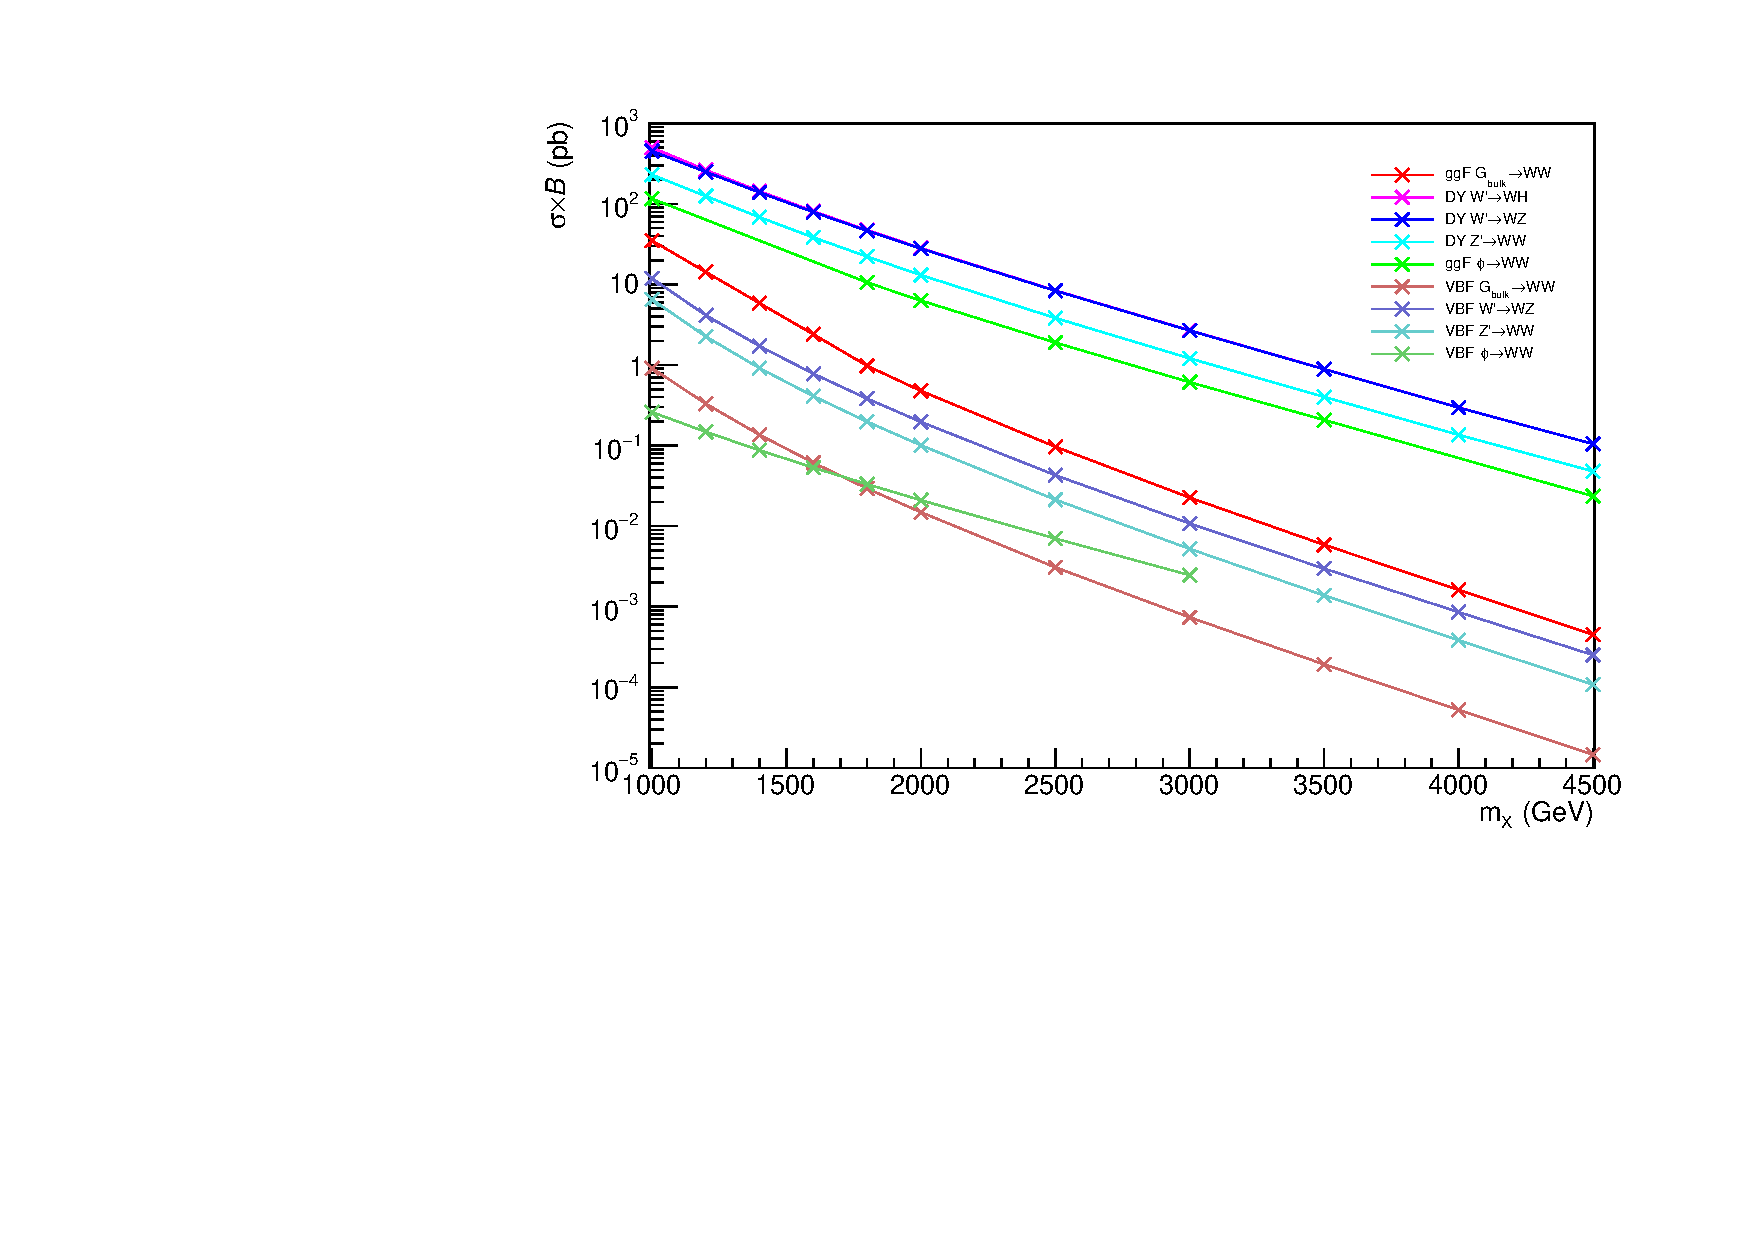
\includegraphics[width=0.75\textwidth]{fig/samples/sigCrossSec.pdf}
  \caption{
    Cross sections multiplied by branching ratios for each of the benchmark signal MC samples as a function of the resonance mass \MX.
  }
  \label{fig:sigCrossSec}
\end{figure}

%\begin{table}[htbp]
%  \centering
%  % !TEX root = ../../thesis.tex
\scriptsize
\begin{tabular}{lrr}
  \hline
  \textbf{Sample name} & $\sigma_{\ggF}(\GBulktoWW)$ [fb] & $B(\WWtolnuqqbarpr)$ \\
  \hline
  \ttfamily /BulkGravToWWToWlepWhad\_narrow\_M-1000\_[SUFFIX] & 35.1 & 0.442  \\
  \ttfamily /BulkGravToWWToWlepWhad\_narrow\_M-1200\_[SUFFIX] & 14.3 & 0.442  \\
  \ttfamily /BulkGravToWWToWlepWhad\_narrow\_M-1400\_[SUFFIX] & 5.86 & 0.442  \\
  \ttfamily /BulkGravToWWToWlepWhad\_narrow\_M-1600\_[SUFFIX] & 2.41 & 0.442  \\
  \ttfamily /BulkGravToWWToWlepWhad\_narrow\_M-1800\_[SUFFIX] & 0.979 & 0.442  \\
  \ttfamily /BulkGravToWWToWlepWhad\_narrow\_M-2000\_[SUFFIX] & 0.478 & 0.442  \\
  \ttfamily /BulkGravToWWToWlepWhad\_narrow\_M-2500\_[SUFFIX] & 0.0967 & 0.442  \\
  \ttfamily /BulkGravToWWToWlepWhad\_narrow\_M-3000\_[SUFFIX] & 0.0226 & 0.442  \\
  \ttfamily /BulkGravToWWToWlepWhad\_narrow\_M-3500\_[SUFFIX] & 0.00586 & 0.442  \\
  \ttfamily /BulkGravToWWToWlepWhad\_narrow\_M-4000\_[SUFFIX] & 0.00162 & 0.442  \\
  \ttfamily /BulkGravToWWToWlepWhad\_narrow\_M-4500\_[SUFFIX] & 0.000451 & 0.442  \\
  \hline
\end{tabular}

%  \caption{
%    Samples for the \ggF\GBulktoWW signal with cross sections and branching ratios.
%    ``\texttt{[SUFFIX]}'' is \texttt{13TeV-madgraph} for the Summer16 campaign, and \texttt{TuneCP5\_13TeV-madgraph-pythia8} for Fall17 and Autumn18.
%  }
%  \label{tab:ggFGBulkToWWSamples}
%\end{table}

%\begin{table}[htbp]
%  \centering
%  % !TEX root = ../../thesis.tex
\scriptsize
\begin{tabular}{lrr}
  \hline
  \textbf{Sample name} & $\sigma_{\VBF}(\GBulktoWW)$ [fb] & $B(\WWtolnuqqbarpr)$ \\
  \hline
  \ttfamily /VBF\_BulkGravToWW\_narrow\_M-1000\_[SUFFIX] &   \\
  \ttfamily /VBF\_BulkGravToWW\_narrow\_M-1200\_[SUFFIX] &   \\
  \ttfamily /VBF\_BulkGravToWW\_narrow\_M-1400\_[SUFFIX] &   \\
  \ttfamily /VBF\_BulkGravToWW\_narrow\_M-1600\_[SUFFIX] &   \\
  \ttfamily /VBF\_BulkGravToWW\_narrow\_M-1800\_[SUFFIX] &   \\
  \ttfamily /VBF\_BulkGravToWW\_narrow\_M-2000\_[SUFFIX] &   \\
  \ttfamily /VBF\_BulkGravToWW\_narrow\_M-2500\_[SUFFIX] &   \\
  \ttfamily /VBF\_BulkGravToWW\_narrow\_M-3000\_[SUFFIX] &   \\
  \ttfamily /VBF\_BulkGravToWW\_narrow\_M-3500\_[SUFFIX] &   \\
  \ttfamily /VBF\_BulkGravToWW\_narrow\_M-4000\_[SUFFIX] &   \\
  \ttfamily /VBF\_BulkGravToWW\_narrow\_M-4500\_[SUFFIX] &   \\
  \hline
\end{tabular}

%  \caption{
%    Samples for the \VBF\GBulktoWW signal with cross sections and branching ratios.
%    ``\texttt{[SUFFIX]}'' is \texttt{13TeV-madgraph-pythia8} for the Summer16 campaign, \texttt{TuneCP5\_13TeV-madgraph} for Fall17, and \texttt{TuneCP5\_PSweights\_13TeV-madgraph} for Autumn18.
%    For Summer16, the prefix is \texttt{VBF\_BulkGravToWWinclusive}.
%  }
%  \label{tab:VBFGBulkToWWSamples}
%\end{table}

%\begin{table}[htbp]
%  \centering
%  % !TEX root = ../../thesis.tex
\scriptsize
\begin{tabular}{lrr}
  \hline
  \textbf{Sample name} & $\sigma_{\ggF}(\RadtoWW)$ [fb] & $B(\WWtolnuqqbarpr)$ \\
  \hline
  \ttfamily /RadionToWW\_narrow\_M-1000\_[SUFFIX] &   \\
  \ttfamily /RadionToWW\_narrow\_M-1200\_[SUFFIX] &   \\
  \ttfamily /RadionToWW\_narrow\_M-1400\_[SUFFIX] &   \\
  \ttfamily /RadionToWW\_narrow\_M-1600\_[SUFFIX] &   \\
  \ttfamily /RadionToWW\_narrow\_M-1800\_[SUFFIX] &   \\
  \ttfamily /RadionToWW\_narrow\_M-2000\_[SUFFIX] &   \\
  \ttfamily /RadionToWW\_narrow\_M-2500\_[SUFFIX] &   \\
  \ttfamily /RadionToWW\_narrow\_M-3000\_[SUFFIX] &   \\
  \ttfamily /RadionToWW\_narrow\_M-3500\_[SUFFIX] &   \\
  \ttfamily /RadionToWW\_narrow\_M-4000\_[SUFFIX] &   \\
  \ttfamily /RadionToWW\_narrow\_M-4500\_[SUFFIX] &   \\
  \hline
\end{tabular}

%  \caption{
%    Samples for the \ggF\RadtoWW signal with cross sections and branching ratios.
%    ``\texttt{[SUFFIX]}'' is \texttt{13TeV-madgraph} for the Summer16 campaign, and \texttt{TuneCP5\_13TeV-madgraph} for Fall17 and Autumn18.
%  }
%  \label{tab:ggFRadToWWSamples}
%\end{table}

%\begin{table}[htbp]
%  \centering
%  % !TEX root = ../../thesis.tex
\scriptsize
\begin{tabular}{lrr}
  \hline
  \textbf{Sample name} & $\sigma_{\VBF}(\RadtoWW)$ [fb] & $B(\WWtolnuqqbarpr)$ \\
  \hline
  \ttfamily /VBF\_RadionToWW\_narrow\_M-1000\_[SUFFIX] &   \\
  \ttfamily /VBF\_RadionToWW\_narrow\_M-1200\_[SUFFIX] &   \\
  \ttfamily /VBF\_RadionToWW\_narrow\_M-1400\_[SUFFIX] &   \\
  \ttfamily /VBF\_RadionToWW\_narrow\_M-1600\_[SUFFIX] &   \\
  \ttfamily /VBF\_RadionToWW\_narrow\_M-1800\_[SUFFIX] &   \\
  \ttfamily /VBF\_RadionToWW\_narrow\_M-2000\_[SUFFIX] &   \\
  \ttfamily /VBF\_RadionToWW\_narrow\_M-2500\_[SUFFIX] &   \\
  \ttfamily /VBF\_RadionToWW\_narrow\_M-3000\_[SUFFIX] &   \\
  \ttfamily /VBF\_RadionToWW\_narrow\_M-3500\_[SUFFIX] &   \\
  \ttfamily /VBF\_RadionToWW\_narrow\_M-4000\_[SUFFIX] &   \\
  \ttfamily /VBF\_RadionToWW\_narrow\_M-4500\_[SUFFIX] &   \\
  \hline
\end{tabular}

%  \caption{
%    Samples for the \VBF\RadtoWW signal with cross sections and branching ratios.
%    ``\texttt{[SUFFIX]}'' is \texttt{13TeV-madgraph} for the Summer16 campaign, \texttt{TuneCP5\_13TeV-madgraph} for Fall17, and \texttt{TuneCP5\_PSweights\_13TeV-madgraph} for Autumn18.
%  }
%  \label{tab:VBFRadToWWSamples}
%\end{table}

%\begin{table}[htbp]
%  \centering
%  % !TEX root = ../../thesis.tex
\scriptsize
\begin{tabular}{lrr}
  \hline
  \textbf{Sample name} & $\sigma_{\DY}(\WprtoWZ)$ [fb] & $B(\WZtolnuqqbar)$ \\
  \hline
  \ttfamily /WprimeToWZToWlepZhad\_narrow\_M-1000\_[SUFFIX] & 454 & 0.229  \\
  \ttfamily /WprimeToWZToWlepZhad\_narrow\_M-1200\_[SUFFIX] & 250 & 0.229  \\
  \ttfamily /WprimeToWZToWlepZhad\_narrow\_M-1400\_[SUFFIX] & 139 & 0.229  \\
  \ttfamily /WprimeToWZToWlepZhad\_narrow\_M-1600\_[SUFFIX] & 79.2 & 0.229  \\
  \ttfamily /WprimeToWZToWlepZhad\_narrow\_M-1800\_[SUFFIX] & 46.5 & 0.229  \\
  \ttfamily /WprimeToWZToWlepZhad\_narrow\_M-2000\_[SUFFIX] & 27.9 & 0.229  \\
  \ttfamily /WprimeToWZToWlepZhad\_narrow\_M-2500\_[SUFFIX] & 8.37 & 0.229  \\
  \ttfamily /WprimeToWZToWlepZhad\_narrow\_M-3000\_[SUFFIX] & 2.68 & 0.229  \\
  \ttfamily /WprimeToWZToWlepZhad\_narrow\_M-3500\_[SUFFIX] & 0.888 & 0.229  \\
  \ttfamily /WprimeToWZToWlepZhad\_narrow\_M-4000\_[SUFFIX] & 0.296 & 0.229  \\
  \ttfamily /WprimeToWZToWlepZhad\_narrow\_M-4500\_[SUFFIX] & 0.105 & 0.229  \\
  \hline
\end{tabular}

%  \caption{
%    Samples for the \DY\WprtoWZ signal with cross sections and branching ratios.
%    ``\texttt{[SUFFIX]}'' is \texttt{13TeV-madgraph} for the Summer16 campaign, and \texttt{TuneCP5\_13TeV-madgraph-pythia8} for Fall17 and Autumn18.
%  }
%  \label{tab:DYWprToWZSamples}
%\end{table}

%\begin{table}[htbp]
%  \centering
%  % !TEX root = ../../thesis.tex
\scriptsize
\begin{tabular}{lrr}
  \hline
  \textbf{Sample name} & $\sigma_{\VBF}(\WprtoWZ)$ [fb] & $B(\WZtolnuqqbar)$ \\
  \hline
  \ttfamily /VBF\_WprimeToWZ\_narrow\_M-1000\_[SUFFIX] & 11.9  \\
  \ttfamily /VBF\_WprimeToWZ\_narrow\_M-1200\_[SUFFIX] & 4.15  \\
  \ttfamily /VBF\_WprimeToWZ\_narrow\_M-1400\_[SUFFIX] & 1.72  \\
  \ttfamily /VBF\_WprimeToWZ\_narrow\_M-1600\_[SUFFIX] & 0.780  \\
  \ttfamily /VBF\_WprimeToWZ\_narrow\_M-1800\_[SUFFIX] & 0.383  \\
  \ttfamily /VBF\_WprimeToWZ\_narrow\_M-2000\_[SUFFIX] & 0.197  \\
  \ttfamily /VBF\_WprimeToWZ\_narrow\_M-2500\_[SUFFIX] & 0.0429  \\
  \ttfamily /VBF\_WprimeToWZ\_narrow\_M-3000\_[SUFFIX] & 0.0108  \\
  \ttfamily /VBF\_WprimeToWZ\_narrow\_M-3500\_[SUFFIX] & 0.00297  \\
  \ttfamily /VBF\_WprimeToWZ\_narrow\_M-4000\_[SUFFIX] & 0.000857  \\
  \ttfamily /VBF\_WprimeToWZ\_narrow\_M-4500\_[SUFFIX] & 0.000251  \\
  \hline
\end{tabular}

%  \caption{
%    Samples for the \VBF\WprtoWZ signal with cross sections and branching ratios.
%    ``\texttt{[SUFFIX]}'' is \texttt{13TeV-madgraph-pythia8} for the Summer16 campaign, \texttt{TuneCP5\_13TeV-madgraph} for Fall17, and \texttt{TuneCP5\_PSweights\_13TeV-madgraph} for Autumn18.
%    For Summer16, the prefix is \texttt{VBF\_WprimeToWZinclusive}.
%  }
%  \label{tab:VBFWprToWZSamples}
%\end{table}

%\begin{table}[htbp]
%  \centering
%  % !TEX root = ../../thesis.tex
\scriptsize
\begin{tabular}{lrr}
  \hline
  \textbf{Sample name} & $\sigma_{\DY}(\WprtoWH)$ [fb] & $B(\WHtolnubbbar)$ \\
  \hline
  \ttfamily /WprimeToWHToWlepHinc\_narrow\_M-1000\_[SUFFIX] & 201 & 0.327  \\
  \ttfamily /WprimeToWHToWlepHinc\_narrow\_M-1200\_[SUFFIX] & 264 & 0.327  \\
  \ttfamily /WprimeToWHToWlepHinc\_narrow\_M-1400\_[SUFFIX] & 144 & 0.327  \\
  \ttfamily /WprimeToWHToWlepHinc\_narrow\_M-1600\_[SUFFIX] & 81.3 & 0.327  \\
  \ttfamily /WprimeToWHToWlepHinc\_narrow\_M-1800\_[SUFFIX] & 47.3 & 0.327  \\
  \ttfamily /WprimeToWHToWlepHinc\_narrow\_M-2000\_[SUFFIX] & 28.3 & 0.327  \\
  \ttfamily /WprimeToWHToWlepHinc\_narrow\_M-2500\_[SUFFIX] & 8.44 & 0.327  \\
  \ttfamily /WprimeToWHToWlepHinc\_narrow\_M-3000\_[SUFFIX] & 2.70 & 0.327  \\
  \ttfamily /WprimeToWHToWlepHinc\_narrow\_M-3500\_[SUFFIX] & 0.892 & 0.327  \\
  \ttfamily /WprimeToWHToWlepHinc\_narrow\_M-4000\_[SUFFIX] & 0.297 & 0.327  \\
  \ttfamily /WprimeToWHToWlepHinc\_narrow\_M-4500\_[SUFFIX] & 0.105 & 0.327  \\
  \hline
\end{tabular}

%  \caption{
%    Samples for the \DY\WprtoWH signal with cross sections and branching ratios.
%    ``\texttt{[SUFFIX]}'' is \texttt{TuneCUETP8M2T4\_13TeV-madgraph-pythia8} for the Summer16 campaign, and \texttt{TuneCP5\_13TeV-madgraph-pythia8} for Fall17 and Autumn18.
%  }
%  \label{tab:DYWprToWHSamples}
%\end{table}

%\begin{table}[htbp]
%  \centering
%  % !TEX root = ../../thesis.tex
\scriptsize
\begin{tabular}{lrr}
  \hline
  \textbf{Sample name} & $\sigma_{\VBF}(\WprtoWH)$ [fb] & $B(\WHtolnubbbar)$ \\
  \hline
\end{tabular}

%  \caption{
%    Samples for the \VBF\WprtoWH signal with cross sections and branching ratios.
%  }
%  \label{tab:VBFWprToWHSamples}
%\end{table}

%\begin{table}[htbp]
%  \centering
%  % !TEX root = ../../thesis.tex
\scriptsize
\begin{tabular}{lrr}
  \hline
  \textbf{Sample name} & $\sigma_{\DY}(\ZprtoWW)$ [fb] & $B(\WWtolnuqqbarpr)$ \\
  \hline
  \ttfamily /ZprimeToWW\_narrow\_M-1000\_[SUFFIX] & 230  \\
  \ttfamily /ZprimeToWW\_narrow\_M-1200\_[SUFFIX] & 125  \\
  \ttfamily /ZprimeToWW\_narrow\_M-1400\_[SUFFIX] & 68.4  \\
  \ttfamily /ZprimeToWW\_narrow\_M-1600\_[SUFFIX] & 38.4  \\
  \ttfamily /ZprimeToWW\_narrow\_M-1800\_[SUFFIX] & 22.2  \\
  \ttfamily /ZprimeToWW\_narrow\_M-2000\_[SUFFIX] & 13.1  \\
  \ttfamily /ZprimeToWW\_narrow\_M-2500\_[SUFFIX] & 3.84  \\
  \ttfamily /ZprimeToWW\_narrow\_M-3000\_[SUFFIX] & 1.21  \\
  \ttfamily /ZprimeToWW\_narrow\_M-3500\_[SUFFIX] & 0.402  \\
  \ttfamily /ZprimeToWW\_narrow\_M-4000\_[SUFFIX] & 0.136  \\
  \ttfamily /ZprimeToWW\_narrow\_M-4500\_[SUFFIX] & 0.048  \\
  \hline
\end{tabular}

%  \caption{
%    Samples for the \DY\ZprtoWW signal with cross sections and branching ratios.
%    ``\texttt{[SUFFIX]}'' is \texttt{13TeV-madgraph} for the Summer16 campaign, and \texttt{TuneCP5\_13TeV-madgraph} for Fall17 and Autumn18.
%  }
%  \label{tab:DYZprToWWSamples}
%\end{table}

%\begin{table}[htbp]
%  \centering
%  % !TEX root = ../../thesis.tex
\scriptsize
\begin{tabular}{lrr}
  \hline
  \textbf{Sample name} & $\sigma_{\VBF}(\ZprtoWW)$ [fb] & $B(\WWtolnuqqbarpr)$ \\
  \hline
  \ttfamily /VBF\_ZprimeToWW\_narrow\_M-1000\_[SUFFIX] & 6.53  \\
  \ttfamily /VBF\_ZprimeToWW\_narrow\_M-1200\_[SUFFIX] & 2.26  \\
  \ttfamily /VBF\_ZprimeToWW\_narrow\_M-1400\_[SUFFIX] & 0.915  \\
  \ttfamily /VBF\_ZprimeToWW\_narrow\_M-1600\_[SUFFIX] & 0.411  \\
  \ttfamily /VBF\_ZprimeToWW\_narrow\_M-1800\_[SUFFIX] & 0.198  \\
  \ttfamily /VBF\_ZprimeToWW\_narrow\_M-2000\_[SUFFIX] & 0.101  \\
  \ttfamily /VBF\_ZprimeToWW\_narrow\_M-2500\_[SUFFIX] & 0.0213  \\
  \ttfamily /VBF\_ZprimeToWW\_narrow\_M-3000\_[SUFFIX] & 0.00522  \\
  \ttfamily /VBF\_ZprimeToWW\_narrow\_M-3500\_[SUFFIX] & 0.00138  \\
  \ttfamily /VBF\_ZprimeToWW\_narrow\_M-4000\_[SUFFIX] & 0.000383  \\
  \ttfamily /VBF\_ZprimeToWW\_narrow\_M-4500\_[SUFFIX] & 0.000108  \\
  \hline
\end{tabular}

%  \caption{
%    Samples for the \VBF\ZprtoWW signal with cross sections and branching ratios.
%    ``\texttt{[SUFFIX]}'' is \texttt{13TeV-madgraph-pythia8} for the Summer16 campaign, \texttt{TuneCP5\_13TeV-madgraph} for Fall17, and \texttt{TuneCP5\_PSweights\_13TeV-madgraph} for Autumn18.
%    For Summer16, the prefix is \texttt{VBF\_ZprimeToWWinclusive}.
%  }
%  \label{tab:VBFZprToWWSamples}
%\end{table}

\subsubsection{Background Samples}

% Background samples
The MC samples used to simulate SM background contributions listed in table~\ref{tab:bkgSamples} along with their cross sections. %~\ref{tab:bkg2016Samples} and \ref{tab:bkg2017Samples} along with their cross sections.
These include the previously mentioned background processes described in the introduction, consisting of $W$+jets, \DY+jets, SM diboson, \bbbar, $t\bar{t}$, single-$t$, and QCD production samples.
The background samples were generated in the same \texttt{RunIISummer16MiniAODv2}, \texttt{RunIIFall17MiniAODv2}, and \texttt{RunIIAutumn18MiniAOD} campaigns as for the signal samples.

\begin{table}
  \centering
  % !TEX root = ../../thesis.tex
\scriptsize
\begin{tabular}{l|l|l}
  \hline
  Category & Sample name & Total cross section [pb] \\
  \hline
  \hline
  \Wjets & \ttfamily WJetsToLNu\_HT-[MASS]\_[SUFFIX] & \\
  & \ttfamily WJetsToLNu\_HT-[MASS]\_[SUFFIX] & \\
  \hline
  \DY+jets & \ttfamily DYJetsToLL\_M-50\_HT-[MASS]\_[SUFFIX] & \\
  & \ttfamily DYJetsToLL\_M-50\_HT-[MASS]\_[SUFFIX] & \\
  \hline
  \WVt & \ttfamily WWToLNuQQ\_[SUFFIX] & 49.997 \\
  & \ttfamily WWToLNuQQ\_NNPDF31\_[SUFFIX] & 43.53 \\
  & \ttfamily WZTo1L1Nu2Q\_[SUFFIX] & 10.71 \\
  & \ttfamily ZZTo2L2Q\_[SUFFIX] & 3.28 \\
  \hline
  \bbbar & \ttfamily WplusH\_HToBB\_WToLNu\_M125\_[SUFFIX] & 0.1585 \\
  & \ttfamily WminusH\_HToBB\_WToLNu\_M125\_[SUFFIX] & 0.1005 \\
  & \ttfamily ZH\_HToBB\_ZToLL\_M125\_[SUFFIX] & 0.0520 \\
  \hline
  $t\bar{t}$ & \ttfamily TT\_TuneCUETP8M2T4\_[SUFFIX] & 831.76 \\
  & \ttfamily TTTo2L2Nu\_TuneCP5\_PSweights\_[SUFFIX] & 87.31448 \\
  & \ttfamily TTToHadronic\_TuneCP5\_PSweights\_[SUFFIX] & 380.094 \\
  & \ttfamily TTToSemiLeptonic\_TuneCP5\_PSweights\_[SUFFIX] & 364.3508 \\
  \hline
  Single-$t$ & \ttfamily ST\_t-channel\_top\_4f\_inclusiveDecays\_[TuneCP5]\_[SUFFIX] & 136.02 \\
  & \ttfamily ST\_t-channel\_antitop\_4f\_inclusiveDecays\_[TuneCP5]\_[SUFFIX] & 80.95 \\
  & \ttfamily ST\_tW\_antitop\_5f\_inclusiveDecays\_[TuneCP5]\_[SUFFIX] & 35.6 \\
  & \ttfamily ST\_tW\_top\_5f\_inclusiveDecays\_[TuneCP5]\_[SUFFIX] & 35.6 \\
  \hline
  QCD & \ttfamily QCD\_HT[MASS]\_Tune[CUETP8M1/CP5]\_[SUFFIX] & \\
  \hline
\end{tabular}

  \caption{
    Background samples used for Run 2 with cross sections.
    Here, ``\texttt{[RANGE]}'' refers to the range of the \texttt{HT} variable, which is the scalar sum of the transverse momenta of all jets in the sample, while ``\texttt{[SUFFIX]}'' refers to various tags denoting the campaign in which the samples were made, such as \texttt{13TeV-madgraph} or \texttt{TuneCP5\_13TeV-madgraph-pythia8}.
    The $W$+jets and \DY+jets samples have \texttt{HT} greater than $100\unit{GeV}$ in several bins, and the QCD samples have \texttt{HT} greater than $500\unit{GeV}$.
  }
  \label{tab:bkgSamples}
\end{table}

%\begin{table}[htbp]
%  \centering
%  % !TEX root = ../../thesis.tex
\scriptsize
\begin{tabular}{lrr}
  \hline
  \textbf{Sample name} & \textbf{Cross section[pb]} \\
  \hline
  \ttfamily WJetsToLNu\_HT-100To200\_TuneCUETP8M1\_13TeV-madgraphMLM-pythia8  & 1345*1.21 \\
  \ttfamily WJetsToLNu\_HT-200To400\_TuneCUETP8M1\_13TeV-madgraphMLM-pythia8 & 359.7*1.21 \\
  \ttfamily WJetsToLNu\_HT-400To600\_TuneCUETP8M1\_13TeV-madgraphMLM-pythia8 & 48.91*1.21 \\
  \ttfamily WJetsToLNu\_HT-600To800\_TuneCUETP8M1\_13TeV-madgraphMLM-pythia8 & 12.05*1.21 \\
  \ttfamily WJetsToLNu\_HT-800To1200\_TuneCUETP8M1\_13TeV-madgraphMLM-pythia8 & 5.501*1.21 \\
  \ttfamily WJetsToLNu\_HT-1200To2500\_TuneCUETP8M1\_13TeV-madgraphMLM-pythia8 & 1.329*1.21 \\
  \ttfamily WJetsToLNu\_HT-2500ToInf\_TuneCUETP8M1\_13TeV-madgraphMLM-pythia8 & 0.03216*1.21 \\
  \hline
  \ttfamily DYJetsToLL\_M-50\_HT-100to200\_TuneCUETP8M1\_13TeV-madgraphMLM-pythia8 & 147.4*1.23 \\
  \ttfamily DYJetsToLL\_M-50\_HT-200to400\_TuneCUETP8M1\_13TeV-madgraphMLM-pythia8 & 40.99*1.23 \\
  \ttfamily DYJetsToLL\_M-50\_HT-400to600\_TuneCUETP8M1\_13TeV-madgraphMLM-pythia8 & 5.678*1.23 \\
  \ttfamily DYJetsToLL\_M-50\_HT-600to800\_TuneCUETP8M1\_13TeV-madgraphMLM-pythia8 & 1.367*1.23 \\
  \ttfamily DYJetsToLL\_M-50\_HT-800to1200\_TuneCUETP8M1\_13TeV-madgraphMLM-pythia8 & 0.6304*1.23 \\
  \ttfamily DYJetsToLL\_M-50\_HT-1200to2500\_TuneCUETP8M1\_13TeV-madgraphMLM-pythia8 & 0.1514*1.23 \\
  \ttfamily DYJetsToLL\_M-50\_HT-2500toInf\_TuneCUETP8M1\_13TeV-madgraphMLM-pythia8 & 003565*1.23 \\
  \hline
  \ttfamily WWToLNuQQ\_13TeV-powheg & 49.997 \\
  \ttfamily WZTo1L1Nu2Q\_13TeV\_amcatnloFXFX\_madspin\_pythia8 & 10.71 \\
  \ttfamily ZZTo2L2Q\_13TeV\_amcatnloFXFX\_madspin\_pythia8 & 3.28 \\
  \hline
  \ttfamily WplusH\_HToBB\_WToLNu\_M125\_13TeV\_powheg\_pythia8 & 0.1585 \\
  \ttfamily WminusH\_HToBB\_WToLNu\_M125\_13TeV\_powheg\_pythia8 & 0.1005 \\
  \ttfamily ZH\_HToBB\_ZToLL\_M125\_13TeV\_powheg\_pythia8 & 0.0520 \\
  \hline
  \ttfamily TT\_TuneCUETP8M2T4\_13TeV-powheg-pythia8 & 831.76 \\
  \hline
  %\ttfamily ST\_s-channel\_4f\_leptonDecays\_13TeV-amcatnlo-pythia8\_TuneCUETP8M1 & 3.68 \\
  \ttfamily ST\_t-channel\_top\_4f\_inclusiveDecays\_13TeV-powhegV2-madspin-pythia8\_TuneCUETP8M1 & 136.02 \\
  \ttfamily ST\_t-channel\_antitop\_4f\_inclusiveDecays\_13TeV-powhegV2-madspin-pythia8\_TuneCUETP8M1 & 80.95 \\
  \ttfamily ST\_tW\_antitop\_5f\_inclusiveDecays\_13TeV-powheg-pythia8\_TuneCUETP8M1 & 35.6 \\
  \ttfamily ST\_tW\_top\_5f\_inclusiveDecays\_13TeV-powheg-pythia8\_TuneCUETP8M1 & 35.6 \\
  \hline
  %\ttfamily QCD\_HT100to200\_TuneCUETP8M1\_13TeV-madgraphMLM-pythia8 & 2.785*1e7 \\
  %\ttfamily QCD\_HT200to300\_TuneCUETP8M1\_13TeV-madgraphMLM-pythia8 & 1717000 \\
  %\ttfamily QCD\_HT300to500\_TuneCUETP8M1\_13TeV-madgraphMLM-pythia8 & 351300 \\
  \ttfamily QCD\_HT500to700\_TuneCUETP8M1\_13TeV-madgraphMLM-pythia8 & 31630 \\
  \ttfamily QCD\_HT700to1000\_TuneCUETP8M1\_13TeV-madgraphMLM-pythia8 & 6802 \\
  \ttfamily QCD\_HT1000to1500\_TuneCUETP8M1\_13TeV-madgraphMLM-pythia8 & 1206 \\
  \ttfamily QCD\_HT1500to2000\_TuneCUETP8M1\_13TeV-madgraphMLM-pythia8 & 120.4 \\
  \ttfamily QCD\_HT2000toInf\_TuneCUETP8M1\_13TeV-madgraphMLM-pythia8 & 25.25 \\
  \hline
\end{tabular}

%  \caption{
%    Background samples used for 2016 with cross sections.
%  }
%  \label{tab:bkg2016Samples}
%\end{table}

%\begin{table}[htbp]
%  \centering
%  % !TEX root = ../../thesis.tex
\scriptsize
\begin{tabular}{lrr}
  \hline
  \textbf{Sample name} & \textbf{Cross section[pb]} \\
  \hline
  \ttfamily WJetsToLNu\_HT-100To200\_TuneCP5\_13TeV-madgraphMLM-pythia8 & 1627.45 \\
  \ttfamily WJetsToLNu\_HT-200To400\_TuneCP5\_13TeV-madgraphMLM-pythia8 & 435.237 \\
  \ttfamily WJetsToLNu\_HT-400To600\_TuneCP5\_13TeV-madgraphMLM-pythia8 & 59.1811 \\
  \ttfamily WJetsToLNu\_HT-600To800\_TuneCP5\_13TeV-madgraphMLM-pythia8 & 14.5805 \\
  \ttfamily WJetsToLNu\_HT-800To1200\_TuneCP5\_13TeV-madgraphMLM-pythia8 & 6.65621 \\
  \ttfamily WJetsToLNu\_HT-1200To2500\_TuneCP5\_13TeV-madgraphMLM-pythia8 & 1.60809 \\
  \ttfamily WJetsToLNu\_HT-2500ToInf\_TuneCP5\_13TeV-madgraphMLM-pythia8 & 0.0389136 \\
  \hline
  \ttfamily DYJetsToLL\_M-50\_HT-100to200\_TuneCP5\_13TeV-madgraphMLM-pythia8 & 174.0 \\
  \ttfamily DYJetsToLL\_M-50\_HT-200to400\_TuneCP5\_13TeV-madgraphMLM-pythia8 & 53.27 \\
  \ttfamily DYJetsToLL\_M-50\_HT-400to600\_TuneCP5\_13TeV-madgraphMLM-pythia8 & 7.79 \\
  \ttfamily DYJetsToLL\_M-50\_HT-600to800\_TuneCP5\_13TeV-madgraphMLM-pythia8 & 1.882 \\
  \ttfamily DYJetsToLL\_M-50\_HT-800to1200\_TuneCP5\_13TeV-madgraphMLM-pythia8 & 0.8729 \\
  \ttfamily DYJetsToLL\_M-50\_HT-1200to2500\_TuneCP5\_13TeV-madgraphMLM-pythia8 & 0.2079 \\
  \ttfamily DYJetsToLL\_M-50\_HT-2500toInf\_TuneCP5\_13TeV-madgraphMLM-pythia8 & 0.003765 \\
  \hline
  \ttfamily WWToLNuQQ\_NNPDF31\_TuneCP5\_13TeV-powheg-pythia8 & 43.53 \\
  \ttfamily WZTo1L1Nu2Q\_13TeV\_amcatnloFXFX\_madspin\_pythia8 & 10.71 \\
  \ttfamily ZZTo2L2Q\_13TeV\_amcatnloFXFX\_madspin\_pythia8 & 3.28 \\
  \hline
  \ttfamily WplusH\_HToBB\_WToLNu\_M125\_13TeV\_powheg\_pythia8 & 0.1585 \\
  \ttfamily WminusH\_HToBB\_WToLNu\_M125\_13TeV\_powheg\_pythia8 & 0.1005 \\
  \ttfamily ZH\_HToBB\_ZToLL\_M125\_13TeV\_powheg\_pythia8 & 0.0520 \\
  \hline
  \ttfamily TTTo2L2Nu\_TuneCP5\_PSweights\_13TeV-powheg-pythia8 & 87.31448 \\
  \ttfamily TTToHadronic\_TuneCP5\_PSweights\_13TeV-powheg-pythia8 & 380.094 \\
  \ttfamily TTToSemiLeptonic\_TuneCP5\_PSweights\_13TeV-powheg-pythia8 & 364.3508 \\
  \hline
  \ttfamily ST\_t-channel\_top\_4f\_inclusiveDecays\_TuneCP5\_13TeV-powhegV2-madspin-pythia8 & 136.02 \\
  \ttfamily ST\_t-channel\_antitop\_4f\_inclusiveDecays\_TuneCP5\_13TeV-powhegV2-madspin-pythia8 & 80.95 \\
  \ttfamily ST\_tW\_antitop\_5f\_inclusiveDecays\_TuneCP5\_13TeV-powheg-pythia8 & 35.6 \\
  \ttfamily ST\_tW\_top\_5f\_inclusiveDecays\_TuneCP5\_13TeV-powheg-pythia8 & 35.6 \\
  \hline
  %\ttfamily QCD\_HT100to200\_TuneCP5\_13TeV-madgraph-pythia8 & 2.785*1e7 \\
  %\ttfamily QCD\_HT200to300\_TuneCP5\_13TeV-madgraph-pythia8 & 1717000 \\
  %\ttfamily QCD\_HT300to500\_TuneCP5\_13TeV-madgraph-pythia8 & 351300 \\
  \ttfamily QCD\_HT500to700\_TuneCP5\_13TeV-madgraph-pythia8 & 31630 \\
  \ttfamily QCD\_HT700to1000\_TuneCP5\_13TeV-madgraph-pythia8 & 6802 \\
  \ttfamily QCD\_HT1000to1500\_TuneCP5\_13TeV-madgraph-pythia8 & 1206 \\
  \ttfamily QCD\_HT1500to2000\_TuneCP5\_13TeV-madgraph-pythia8 & 120.4 \\
  \ttfamily QCD\_HT2000toInf\_TuneCP5\_13TeV-madgraph-pythia8 & 25.25 \\
  \hline
\end{tabular}

%  \caption{
%    Background samples used for 2017 and 2018 with cross sections.
%  }
%  \label{tab:bkg2017Samples}
%\end{table}
